\documentclass[12pt]{article}

% All the packages used.
\usepackage[margin=1.0in]{geometry}
\usepackage{pbox}
\usepackage{array}
\usepackage{multicol}
\usepackage{graphicx}
\graphicspath{ {Images/} }
\usepackage{amsmath}                       % Use normal text in math mode.
\usepackage[font={footnotesize}]{caption}  % Determine size of captions.

\usepackage{tikz}                          % Draw diagrams
\usetikzlibrary{shapes.geometric, arrows}

\usepackage{hyperref}                      % Hyperlink.

\begin{document}

% Title page.
\begin{center}
  \vspace*{1in}
  \textbf{\LARGE{BPM Detector (Android)}} \\
  \large{Final Report \\
  Duc Dao \\
  CSC 492, Fall 2017 \\
  Computer Science and Software Engineering Department \\
  College of Engineering\\
  California Polytechnic State University, San Luis Obispo} \\
\end{center}

% Abstract. Must be around 100 to 200 words.
\begin{center}
  \vspace*{2in}
  \textbf{Abstract} \\
\end{center}
The BPM Detector is an Android application that detects the tempo or beats-per-minute (BPM) for a band conductor's conducting. Generally, the conductor moves their arms in a predictable pattern in order to maintain the band's synchronization, acting similarly to a metronome. The purpose of this application is to provide a tool for concert and marching band conductors to detect their precise tempo while conducting. This will help them determine how well they are coordinating the band and whether they need to adjust their tempo.  

\newpage

\tableofcontents

\newpage

% ================================================================================
\section{Introduction}
\subsection{Purpose}
This document is the culmination of all my work for CSC 491 and 492 for \textbf{BPM Detector}, an Android application that detects the beats-per-minute of a conductor's tempo while conducting. The main purpose of the BPM Detector is to aid conductors in seeing how well they are conducting the band and determine whether they need to make adjustments or not. This will benefit marching bands because these types of bands are generally more sensitive to tempo inconsistencies compared to other types of bands.

\subsection{Document Conventions} 
\begin{center}
\Large \textbf{1. Main Section} \\
\large \textbf{1.1 Subsection} \\
\normalsize \textbf{1.1.1 Minor Subsection} \\
\normalsize Body text \\
\tiny References \\
\end{center}

\subsection{Intended Audience}
The intended audience for this document includes:
\begin{itemize}
	\item Developers
    \item Advisors
    \item Musically Inclined Users
 \end{itemize}

\subsubsection{Developers}
Along as a the Final Report for my senior project, this document will serve as a repository of my thoughts and work on BPM Detector, which maybe useful to other developers, including my future self.

\subsubsection{Advisors}
Advisors include:
\begin{itemize}
	\item My senior project advisor, Professor Franz Kurfess
    \item All other resources that aid in my project which may include other professors, students, and other developers
 \end{itemize}

\subsubsection{Musically Inclined Users}
Users that have knowledge and capability of conducting a song may find this project useful for them. This includes, but is not limited to:
\begin{itemize}
	\item Band directors
    \item Drum majors, student conductors
    \item Professors in the Music department
 \end{itemize}

% ================================================================================
\section{Overall Description}
\subsection{Background}
In the context of music ensembles, conducting is the act of directing the group in order to synchronize various components of the band and the performance. Members rely on the conductor to initiate the piece/song that they are performing, set the beats-per-minute or tempo of the song, cue points of interest in the piece, and other musical duties. 
\\
\\
With regards to the tempo, there are no applications to automatically detect the conductor's BPM while they are conducting. Existing solutions on the Google Play Store have users tap on the screen to manually calculate the BPM. Metronome applications only sound off the BPM by setting a certain tempo, or listening to the environment.

\subsection{Problem}
In marching and concert bands, there needs to be some sort of method to synchronize all the members of the band so that they play, rest, and breathe at the appropriate time. This synchronization is typically done by a person such as a conductor, director, or drum major. The conductor synchronizes the band by moving their arm(s) in a predictable pattern in order to maintain the music's tempo. Periodically, bands may mistakenly change tempos not at the fault of the conductor. This becomes hard to identify depending on the song.
\\
\\
Currently, there are no applications to automatically detect the conductor's BPM while they are conducting. Existing solutions on the Google Play Store have users tap on the screen to manually calculate the BPM and metronome applications only sound off the BPM by setting a certain tempo, or listening to the environment.  

\subsection{Solution}
My solution is an Android Wear application that will automatically detect the BPM of the conductor's conducting pattern. The application will utilize the smartwatch's accelerator to calculate the BPM in real-time.

\subsection{Product Functionality}
BPM Detector's will perform one major function: to automatically detect the conductor's tempo while they are conducting.

\subsection{User Class and Their Characteristics}
BPM Detector will be used by one general user class: conductors. Conductors' experiences varies from person to person but all of them generally have knowledge of:
\begin{itemize}
	\item Conducting patterns
    \item Feeling of tempos
    \item Technicalities of the song they are conducting
 \end{itemize}

\subsection{Operating Environment}
BPM Detector will be an Android application running on a smartwatch with at least Android Wear 2.0. The smartwatch requires a Bluetooth connection to an Android phone running at least 6.0 Marshmallow.

\section{External Interface Requirements}
\subsection{User Interfaces}
Users of BPM Detector will interact with the UI of the Android Wear smartwatch. Users will be able to:
\begin{itemize}
	\item Start the BPM detection
    \item Stop the BPM detection
    \item View past detections
\end{itemize}
BPM Detector will utilize elements from Material Design, a design language developed by Google. 

\subsection{Hardware Interfaces}
BPM Detector will be installed on the smartwatch. With the edition of Android Wear to 2.0 (from 1.5), Google has encouraged the use of standalone applications on Android Wear smartwatches.

\subsection{Software Interfaces}
The smartwatch will have the capacity to initiate the BPM detection. During detection, the smartwatch must be able to interpret data from the sensors of the smartwatch and output a number representing the BPM.

\section{Functional Requirements}
BPM Detector functional requirements include the following use cases:
\begin{enumerate}
	\item Starting BPM detection
    \item Stopping BPM detection
    \item Viewing past detections
 \end{enumerate}

\subsection{Starting BPM Detection}
\begin{center}
  \begin{tabular}{ |p{2.5in}|p{3in}| }
  \hline
  \textbf{Use Case ID} & 1 \\[.25in] 
  \hline
  \textbf{Name} & Starting BPM Detection\\[.25in] 
  \hline 
  \textbf{Description} & The act of starting the tempo detection. \\[.25in] 
  \hline 
  \textbf{Preconditions} & User must have the smartwatch on their wrist and the application launched. \\
  \hline
  \textbf{Postconditions} & None \\[.25in] 
  \hline
  \textbf{Priority} & High \\[.25in] 
  \hline 
  \textbf{Frequency of Use} & High \\[.25in] 
  \hline 
  \textbf{Normal Course} & User commences tempo detection. \\[.25in] 
  \hline 
  \textbf{Actor Action} \newline \newline 
  1. User selects "DETECT" on either the smartwatch or smartphone.
  & \textbf{System Responses} \newline \newline
  2. Smartwatch receives initiation and tells sensors to retrieve information in real-time. \newline
  3. Smartwatch interprets sensor information and calculates a BPM number. \newline
  4. Smartwatch displays BPM. \\[.25in]
  \hline
  \end{tabular}
\end{center}

\subsection{Stopping BPM Detection}
\begin{center}
  \begin{tabular}{ |p{2.5in}|p{3in}| }
  \hline
  \textbf{Use Case ID} & 2 \\[.25in] 
  \hline
  \textbf{Name} & Stopping BPM Detection \\[.25in] 
  \hline 
  \textbf{Description} & The act of stopping the tempo detection. \\[.25in] 
  \hline 
  \textbf{Preconditions} & User started the application and initiated detection. Smartwatch is currently detecting BPM. \\
  \hline
  \textbf{Postconditions} & Smartwatch has stopped detecting BPM. \\[.25in] 
  \hline
  \textbf{Priority} & High \\[.25in] 
  \hline 
  \textbf{Frequency of Use} & High \\[.25in] 
  \hline 
  \textbf{Normal Course} & User ceases tempo detection. \\[.25in] 
  \hline 
  \textbf{Actor Action} \newline \newline 
  1. User selects "STOP" on the smartwatch.
  & \textbf{System Responses} \newline \newline
  2. Smartwatch receives cease selection and tells sensors to stop retrieving information in real-time. \newline
  3. Smartwatch asks user if they want to save their detection data for future viewing. \\[.25in] 
  \hline
  \end{tabular}
\end{center}
  
\subsection{Viewing Past Detections}
\begin{center}  
  \begin{tabular}{ |p{2.5in}|p{3in}| }
  \hline
  \textbf{Use Case ID} & 3 \\[.25in] 
  \hline
  \textbf{Name} & Viewing Past Detections \\[.25in] 
  \hline 
  \textbf{Description} & Viewing detections user made in the past. \\[.25in] 
  \hline 
  \textbf{Preconditions} & 
     User has done at least one detection and is saved correctly. \\
  \hline
  \textbf{Postconditions} & None \\[.25in] 
  \hline
  \textbf{Priority} & Low \\[.25in] 
  \hline 
  \textbf{Frequency of Use} & Medium \\[.25in] 
  \hline 
  \textbf{Normal Course} & User views past detections. \\[.25in] 
  \hline 
  \textbf{Actor Action} \newline \newline 
  1. User selects appropriate page containing detection information. \newline \newline
  3. User selects which past detection they want to view in detail. \newline
  & \textbf{System Responses} \newline \newline
  2. Smartwatch receives selection and takes user to a listing of past detections. \newline \newline
  4. Smartwatch displays past detection the user has selected and displays information associated with that detection. \\[.25in] 
  \hline
  \end{tabular}
\end{center}

% ================================================================================
\section{Non-Functional Requirements}
\subsection{Performance Requirements}
All actions performed in the application must take a reasonable amount of time; the faster, the better. The goal is to keep all requests made (starting, stopping, viewing) under 2.5 seconds in terms of response time. To achieve this, the developer must implement the application with consideration to the smartwatch's limited resources.

\subsection{Safety Requirements}
During detection, the smartwatch's temperature cannot exceed 110 °F. To prevent this, the developer must be able to utilize the smartwatch's limited resources efficiently.

% ================================================================================
\section{Development Tools}
\subsection{Software}
\subsubsection{Android Studio}
BPM Detector was developed on Android Studio 3.0.1, an integrated development environment (IDE) made specifically for Android, built-in on JetBrains' IntelliJ IDEA.
\\
\\
I used Android API 27 (codenamed Android 8.1 Oreo) as the target software development kit (SDK) version and Android API 23 (codenamed Android 6.0 Marshmallow) as the minimum SDK version. Java 8 was the implementation language utilized.

\subsection{Hardware}
\subsubsection{Windows 10 PC}
Android Studio ran on a Windows 10 PC with the following specifications:
\begin{itemize}
\item Central Processing Unit (CPU): Intel Core i5 6400 @ 2.7GHz
\item Graphics Processing Unit (GPU): Asus GeForce GTX 780 3GB DirectCU II
\item Motherboard: MSI H110I PRO AC Mini ITX LGA 1151
\item Memory (RAM): Kingston HyperX Fury 8GB DDR4-2133
\item Storage: SanDisk Ultra II 480GB, Western Digital Back 2TB
\item Power Supply: Corsair RMx 650W 80+ Gold ATX
\end{itemize}

\subsubsection{Moto 360}
A second generation, 42mm Moto 360 was used to load and test BPM Detector. The Moto 360 has the following specifications:
\begin{itemize}
	\item Chipset: 1.2 GHz quad-core Qualcomm® Snapdragon™ 400 CPU
    \item Memory (RAM): 2 GB
    \item Storage: 4GB
    \item Connectivity: Bluetooth 4.0, LE, aptX
 \end{itemize}

\newpage

% ================================================================================
\section{Implementation Theory}
\subsection{Beat Detection}
In music, most songs can be broken down into beats of 4 (which I'll refer to as \textbf{4/4}). In 4/4, there are four points a conductor must "hit" in physical space in front of them.

\begin{figure}[h!]
\begin{center}
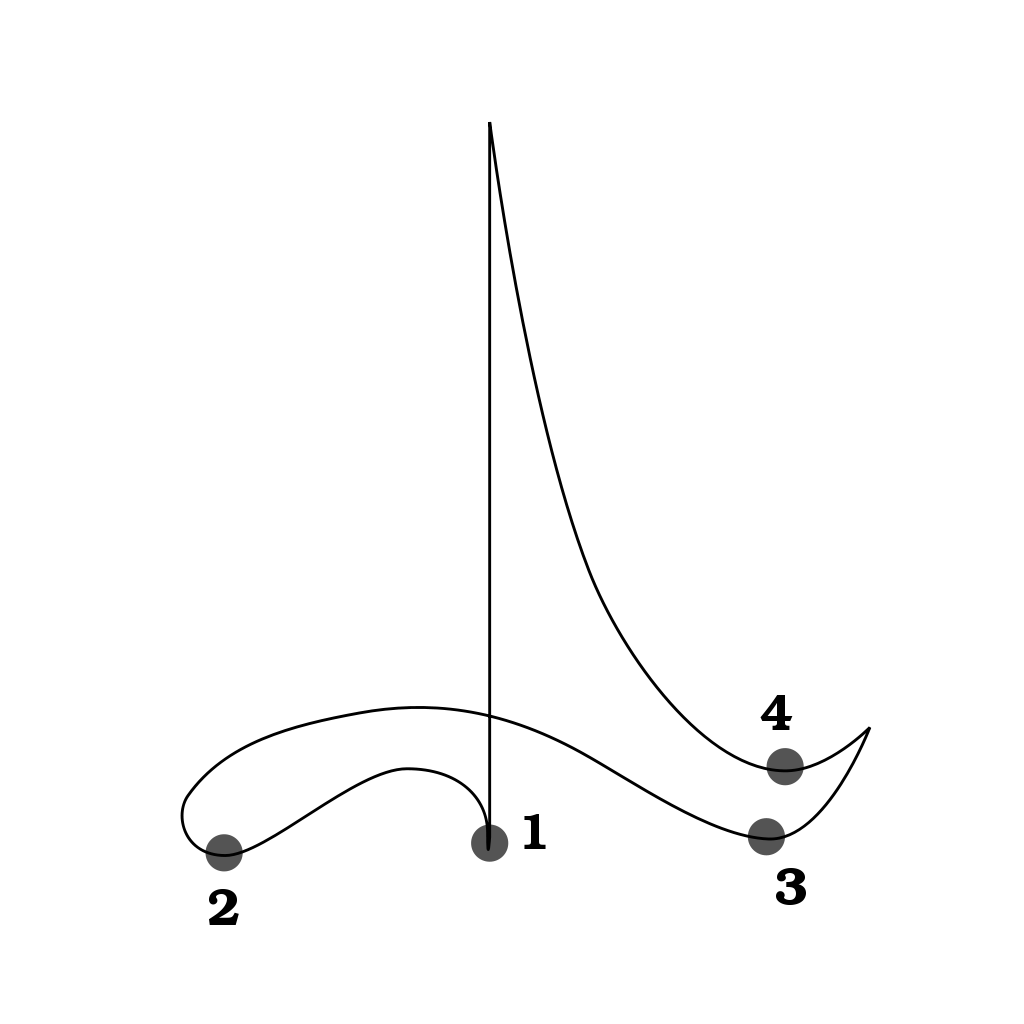
\includegraphics[width=.5\textwidth]{4-4.png}
\caption{The 4 beats the conductor must "hit." 4/4 is referred to as a \textbf{time signature}.}
\tiny{Image Source: \href{https://upload.wikimedia.org/wikipedia/commons/thumb/9/94/Conducting-44time.svg/1024px-Conducting-44time.svg.png}{https://upload.wikimedia.org/wikipedia/commons/thumb/9/94/Conducting-44time.svg/1024px-Conducting-44time.svg.png}}
\label{fig:4-4}
\end{center}
\end{figure}

When a person is conducting, their arms will accelerate up and down rhythmically. Going from beat 1 to 2, most conductors will hit 1, and sharply accelerate their movement in a very minuscule time interval to hit beat 2. During this time interval, the acceleration will increase very rapidly until beat 2 is hit. When beat 2 is hit, the acceleration will instantaneously drop close to 0. This cycle of increasing acceleration in a small time frame followed by a nearly instantaneous acceleration down to 0 happens between every beat. In the context of 4/4, it happens between beats: 
\begin{itemize}
\item 1 to 2
\item 2 to 3
\item 3 to 4
\item 4 to 1
\item 1 to 2...(and so on)
\end{itemize}  

Using this observation, you can generate a graph that has periodic peaks. These peaks occur between the end of the sharply increasing acceleration and the beginning of the near instantaneous acceleration decrease to near 0. These peaks can be identified as beats because the peaks occur when the conductor "hits" a beat in their conducting pattern, the end of the sharp acceleration increase.

\begin{figure}[h!]
\begin{center}
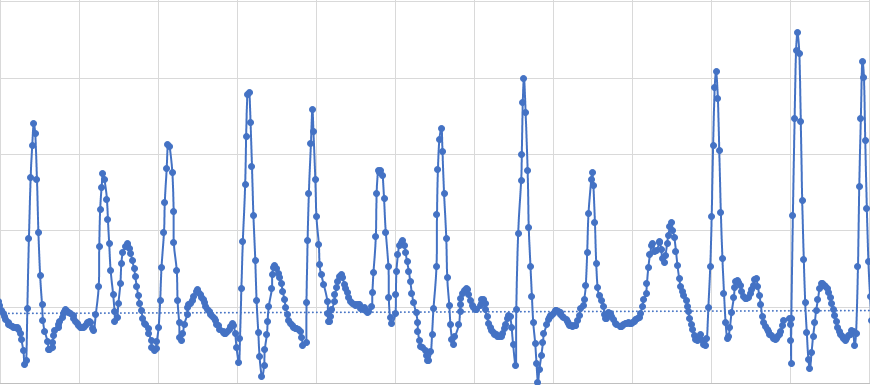
\includegraphics[width=.75\textwidth]{graph1.png}
\caption{A graph generated from conducting UCLA Bruin Marching Band's rendition of "Word Up" while holding my phone. \textbf{X-axis} represents \textbf{time}, \textbf{y-axis} represents \textbf{total linear acceleration}.}
\tiny{Word Up Source: \href{https://www.youtube.com/watch?v=BkRbJ20C72I}{https://www.youtube.com/watch?v=BkRbJ20C72I}}
\label{fig:graph1}
\end{center}
\end{figure}

\subsection{Acceleration}
During our acceleration calculation, gravity is an undesirable variable that could skew our results. To resolve this, we need to use \textbf{linear acceleration}, which accounts for gravity exclusion. Because we have to account for acceleration along the x, y, and z-axis, calculating \textbf{total linear acceleration} will be needed. Total linear acceleration is necessary to account for movement in three dimensional space.

\begin{figure}[h!]
\[\sqrt[]{x^2 + y^2 + z^2}\]
\caption{Formula to calculate total linear acceleration where x, y, and z are the accelerations for each respective axis.}
\label{TLA}
\end{figure}

\subsection{Beats-Per-Minute Calculation}
Knowing when the beats (peaks) occur in the graph shown in Figure~\ref{fig:graph1} allows us to calculate the BPM. By knowing when the beats occurs, you can determine the \textbf{time interval between each beat}. Once you know this time interval, you can figure out how many of these time intervals can fit inside 60 seconds by dividing 60 by some time interval. This means a song that has a BPM of 120 will have a time interval between each beat of .5 seconds, 2 beats a second. \\

\begin{figure}[h!]
\[\ \text{BPM = }\frac{60 \text{ seconds}}{\text{time interval between each beat}}\]
\caption{Formula to calculate the BPM.}
\label{fig:bpm1}
\end{figure}

To stabilize the BPM calculation and make it more accurate, we can take the average of a set of time intervals. This is under the assumption that the BPM of the song remains constant. This would not work if the song changes tempo because past calculations would affect the current one. If that's the case, we must resort to the formula in Figure~\ref{fig:bpm1}.

\begin{figure}[h!]
\[\ \text{BPM = }\frac{60 \text{ seconds}}{\overline{ \text{(time interval between each beat)} }}\]
\caption{Same formula from Figure~\ref{fig:bpm1} but using an average time interval.}
\label{fig:bpm2}
\end{figure}

\begin{figure}[h!]
\begin{center}
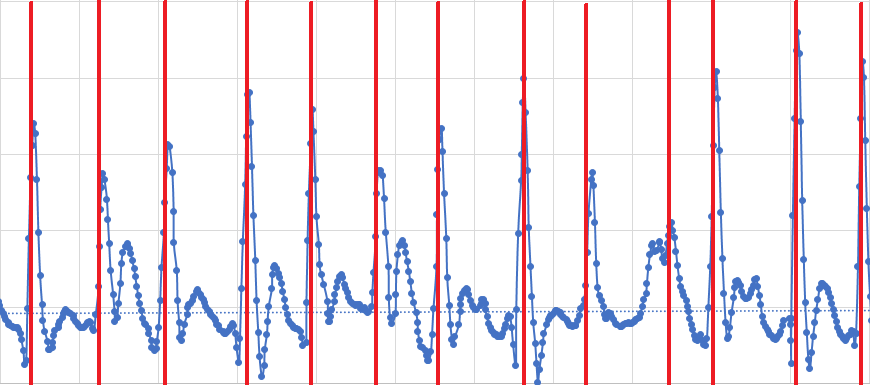
\includegraphics[width=.75\textwidth]{graph2.png}
\caption{The same graph from Figure~\ref{fig:graph1} but with the peaks marked in red. Marking the peaks also makes the time interval between each beat more apparent. Note that there are false positive peaks caused by the conducting style of the user.}
\label{fig:graph}
\end{center}
\end{figure}

% ================================================================================
\section{Software Implementation}
Android consist of many \textbf{activities}, a component that provides a screen for the user to interact with. Every activity has a method called \texttt{onCreate} which serves as the starting point. When switching activities, an \texttt{Intent} is used to describe some operation to perform when making the transition. \\

My implementation can be found \href{https://github.com/ducdao/BPM-Detector}{here}, or at https://github.com/ducdao/BPM-Detector.

\subsection{Activities}
\subsubsection{MainActivity}
\texttt{MainActivity} is the initial starting point for BPM Detector. It contains most of the application code including:
\begin{itemize}
\item UI elements (labels, button colors)
\item Sensor logic
\item Beat detection logic
\item Beats-per-minute calculation
\end{itemize}

\subsubsection{QuerySaveActivity}
\texttt{QuerySaveActivity} gets called by \texttt{MainActivity} after the user stops the detection. This initiates a new screen asking the user if they want to save or delete the most recent detection. 

\subsubsection{ConfirmationActivity}
\texttt{ConfirmationActivity} is a class that's defined in the Android Wearable library, meant to standardize confirmation responses.

% ================================================================================
\section{Testing}
The kinesthetic nature of BPM Detector requires testing the application physically through conducting. Development turnaround (the time between compiling the application and transferring it to my Moto 360) was a massive overhead during testing, taking as long as 2 minutes from clicking the Run button to launching the application. I would spend a minute or two waiting for it to compile, only to having the application crash. This made functional testing impractical.

% ================================================================================
\section{Development Screenshots}
\subsection{Accelerometer - Linear Aceeleration in X, Y, and Z Axes}
\begin{center}
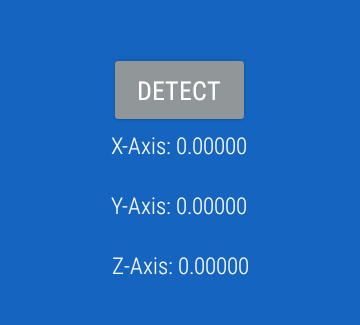
\includegraphics[width=.4\textwidth]{bpm1.png}
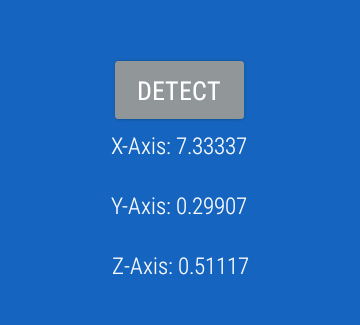
\includegraphics[width=.4\textwidth]{bpm2.png}
\end{center}
\subsection{Start Detection Time + Duration of Detection}
\begin{center}
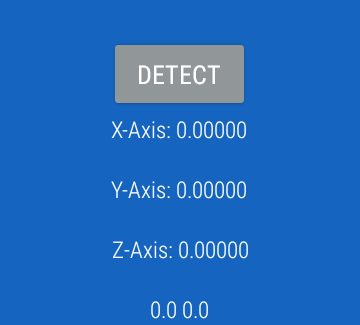
\includegraphics[width=.4\textwidth]{bpm3.png}
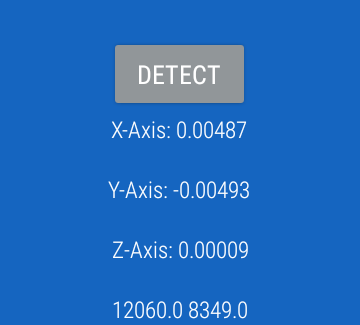
\includegraphics[width=.4\textwidth]{bpm4.png}
\end{center}
\subsection{Calculated Total Acceleration}
\begin{center}
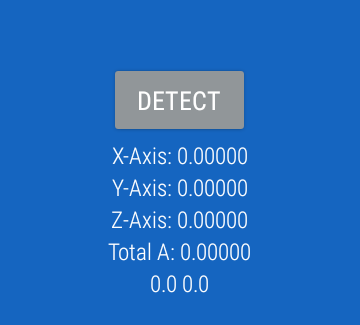
\includegraphics[width=.4\textwidth]{bpm5.png}
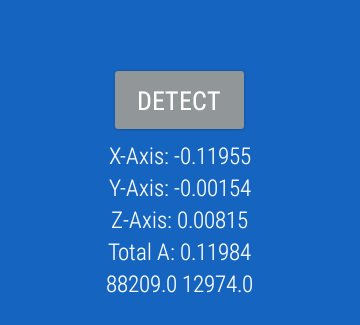
\includegraphics[width=.4\textwidth]{bpm6.png}
\end{center}
\subsection{Started BPM Calculation}
\begin{center}
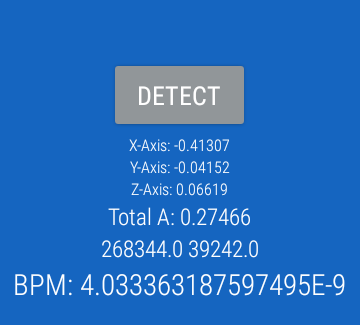
\includegraphics[width=.4\textwidth]{bpm7.png}
\end{center}
\subsection{Removed X, Y, Z Values from UI}
\begin{center}
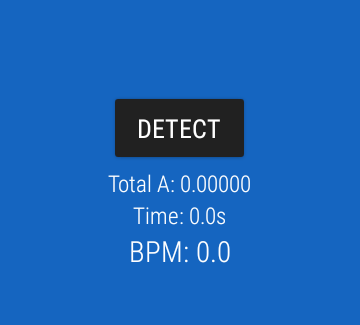
\includegraphics[width=.4\textwidth]{bpm8.png}
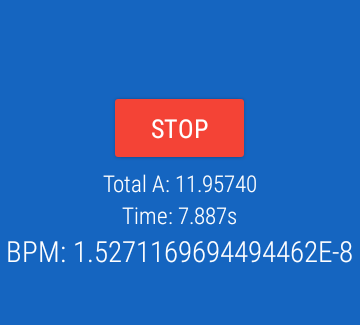
\includegraphics[width=.4\textwidth]{bpm9.png}
\end{center}
\subsection{Confirmation Page for Saving Latest Detection Information}
\begin{center}
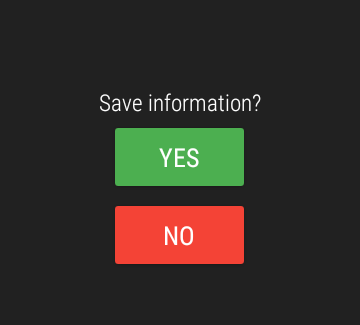
\includegraphics[width=.4\textwidth]{bpm10.png}
\end{center}
\subsection{UI Changes}
\begin{center}
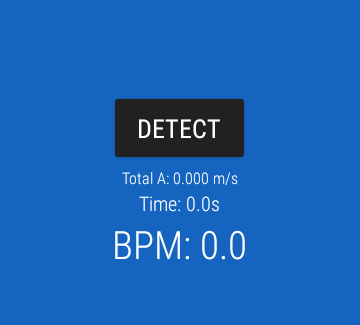
\includegraphics[width=.4\textwidth]{bpm11.png}
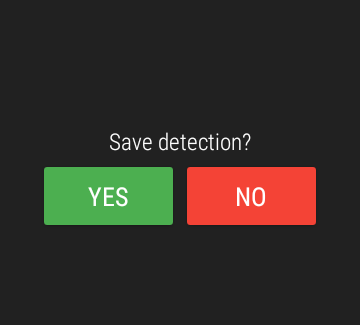
\includegraphics[width=.4\textwidth]{bpm12.png}
\end{center}

% ================================================================================
\section{Problems}
\subsection{Testing}
As said in the Testing section, development turnaround was long. This made development rather tedious, so I had to make sure what I was programming was as bug free as possible to prevent another repetition of waiting only for the application to crash.

\subsection{Moto 360 Display}
During CSC 491, my Moto 360's screen started to act up. Only the top portion of the screen was actually displaying anything. This was problematic because the Moto 360 screen is already really small. Having half the screen broken would hinder UI testing. At first, I wanted to replace the screen but finding spare parts, let along the screen, was difficult. I ended up just purchasing another second generation Moto 360 for as cheap as possible.

\subsection{Real-time Detection}
Doing the calculation in real-time proved to be the most challenging part of the project. Saving every total linear acceleration in a TreeMap would cause the application to actually use all of my Moto 360's RAM and throw a OutOfMemoryError exception. Unfortunately, I couldn't get to debug this in time.

% ================================================================================
\section{Prospective Improvements}
\subsection{Frontend}
\begin{itemize}
\item An Android phone counterpart so that the user can see the BPM in real-time
\item Fully implement \texttt{RecyclerView} to render saved detections
\item Graph view of detections
\item Conducting aid in the form of periodic vibrations
\end{itemize}

\subsection{Backend}
\begin{itemize}
\item Optimize beat detection to increase application accuracy and robustness
\item Account for tempo changes, most likely changing Figure~\ref{fig:bpm2} back to Figure~\ref{fig:bpm1}
\item Load detection data to some data store like Firebase
\end{itemize}

% ================================================================================
\section{Conclusion}
In conclusion, developing BPM Detector has been a fantastic and practical experience for me. I always wanted to do Android development ever since my first year at Cal Poly but always felt overwhelmed by the Android framework. Fast forward a few years and I've gained enough experience through classes and other projects to really dive into Android development head first. The Android platform has really matured over the years, making documentation reading and problem solving much easier than previous years. For the time being, I plan to continue development on BPM Detector to build an application that is not only practical to me but for other entities such as bands as well. I hope to bring this experience developing BPM Detector into my career as a prospective Android developer.

\end{document}